\chapter{Problemas de rutas}
\label{chap4}
\ifpdf
  \graphicspath{{Chapter4/Chapter4Figs/PNG/}{Chapter4/Chapter4Figs/PDF/}{Chapter4/Chapter4Figs/}}
\else
  \graphicspath{{Chapter4/Chapter4Figs/EPS/}{Chapter4/Chapter4Figs/}}
\fi

\markboth{\hfill \thechapter. Problemas de rutas}{\hfill \thechapter. Problemas de rutas}

Los problemas de rutas son todos aquellos de optimización que se plantean cuando existen unos clientes que demandan un servicio y se debe encontrar la mejor ruta para satisfacerles. Algunos ejemplos típicos son el reparto de correo, la recogida de basura o el transporte escolar, también sirve para modelar otras situaciones como la producción de circuitos electrónicos integrados o la secuenciación de tareas \citep{CalvinoM2011CooperacionPanoramica}. En este capítulo se presentan conceptos básicos de los problemas de rutas y de optimización.

Los problemas de rutas se modelan en un grafo G = (V, A), donde existe un coste no negativo asociado a los arcos y aristas del grafo. Estos problemas se dividen en dos clases: los problemas de rutas por nodos y los problemas de rutas por arcos, que se muestran en el Tabla \ref{table:calsifiacionProblemasRutas}. En el primero de los casos, la ruta óptima a determinar debe visitar todos los nodos, mientras que en el segundo, se deben recorrer todos los arcos del grafo que define el problema. En otras palabras, en los problemas sobre los nodos se entiende que cada cliente está representado por un nodo mientras que en los problemas sobre los arcos se entiende que los arcos son calles que deben ser visitadas \citep{CalvinoM2011CooperacionPanoramica}.

\begin{table}[H]
\caption{Clasificación de problemas de ruta. [Fuente: \cite{CalvinoM2011CooperacionPanoramica}] }
\centering 
\begin{tabular}{cccc}
\hline
Demanda                & \begin{tabular}[c]{@{}c@{}}Restricciones\\ de capacidad\end{tabular} & Nombre habitual del problema                                                                          & Otras restricciones   \\ \hline
\multirow{2}{*}{Nodos} & NO                                                                   & \begin{tabular}[c]{@{}c@{}}Problema del Vendedor Viajante\\ TSP\end{tabular}                          &                       \\ \cline{2-3}
                      & SÍ                                                                   & \begin{tabular}[c]{@{}c@{}}Problema de rutas de vehículos\\ VRP\end{tabular}                          & Recogida/distribución \\ \hline
\multirow{3}{*}{Arcos} & \multirow{2}{*}{NO}                                                  & \begin{tabular}[c]{@{}c@{}}Una componente conexa\\ (Problema del Cartero Chino CPP)\end{tabular}      & Ventanas de tiempo    \\ \cline{3-3}
                      &                                                                      & \begin{tabular}[c]{@{}c@{}}Varias componentes conexas\\ (Problema del Cartero Rural RPP)\end{tabular} & Otras                 \\ \cline{2-3}
                      & SÍ                                                                   & \begin{tabular}[c]{@{}c@{}}Problema de rutas con capacidades\\ CARP\end{tabular}                      &                       \\ \hline
\end{tabular}
\label{table:calsifiacionProblemasRutas}
\end{table}

\section{Problemas de ruta por arcos}

Los problemas de ruta sobre arcos tienen su origen en el siglo XVIII, en la ciudad de Königsberg, donde un río atravesaba la ciudad dividiendo la misma en varias partes, para conectar las partes se contaba con siete puentes (ver Figura \ref{fig:puentesKonigsberg}). Los ciudadanos se preguntaban si es que se podía atravesar todos los puentes pasando sólo una vez por cada uno de ellos.

\begin{figure}[H]
\centerline{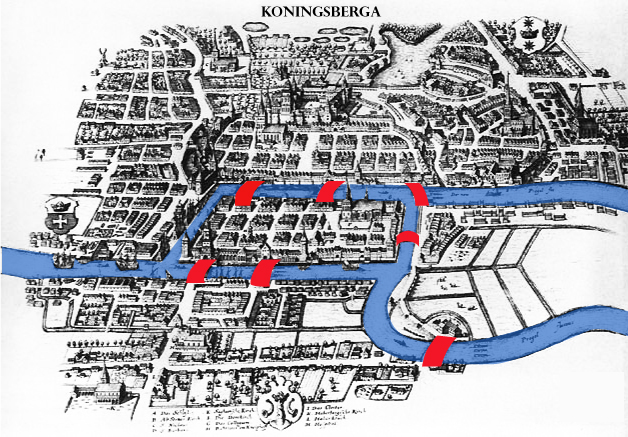
\includegraphics[width=\textwidth]{Konigsberg_bridges.png}}
\caption{Los puentes de Königsberg. [Fuente: \citep{KonigsbergBridges}]}
\label{fig:puentesKonigsberg}
\end{figure}

Leonhard Euler demostró que no era posible, formuló una versión generalizada del problema que establece lo siguiente: si hay dos nodos de grado impar en un grafo, es posible encontrar un camino que atraviese todos los puentes exactamente una vez, empezando en uno de esos nodos y terminando en el otro, esto se conoce como camino euleriano. Si no hay nodos de grado impar, tal camino existe partiendo desde cualquier nodo y terminando en el mismo, esto se conoce como ciclo euleriano. 

En la Figura \ref{fig:grafoPuentesKonigsberg} se observa una representación del grafo de los puentes, en donde cada arco representa a cada uno de ellos. Como los vértices tienen un número de grado impar, es imposible realizar lo que los ciudadanos se planteaban.

\begin{figure}[H]
\centerline{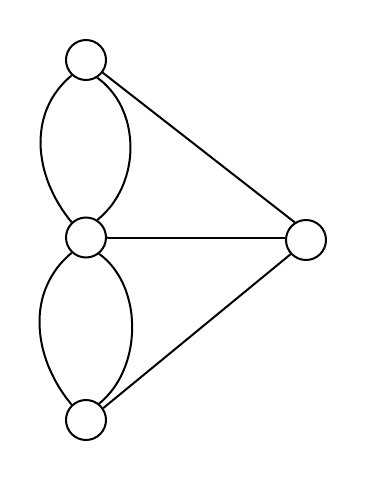
\includegraphics[width=0.6\textwidth]{puentes_grafo.png}}
\caption{Representación del grafo de los puentes de Konigsberg.}
\label{fig:grafoPuentesKonigsberg}
\end{figure}

\subsection{Problema del Cartero Chino (CPP)}

El problema del cartero chino, también conocido como problema del circuito del cartero, el problema de los correos o problema de la inspección y selección de rutas, es el primer problema de rutas por arcos en el que se plantea la posibilidad de construir un ciclo euleriano con coste óptimo \citep{YordaPerez2014ElChino}. 

El problema original dio lugar a multitud de variantes:

\begin{itemize}
    \item CPP en un grafo no dirigido.
    \item CPP en un grafo dirigido.
    \item CPP en un grafo mixto.
\end{itemize}

\subsection{Problema del Cartero Rural (RPP)}

En algunos casos no es necesario atravesar todas las aristas, o arcos, sino solo un subconjunto de ellos (que denominaremos como aristas o arcos requeridos y denotaremos por $A_R$). Sea el grafo G(V, A) un grafo conexo con costes asociados no negativos, en este problema nos interesa definir un ciclo que recorra todos los arcos y/o aristas de $A_R$ al menos una vez. El RPP puede plantearse como un cartero que tiene que repartir el correo en varios pueblos, tiene que recorrer todas las calles de los pueblos, pero no todas las carreteras que los unen.

En general se trata de un problema NP-duro, sin embargo si es un grafo estrictamente dirigido o no dirigido se puede resolver en tiempo polinómico siempre y cuando el subgrafo formado por las aristas o arcos requeridos sea fuertemente conexo. Sus variantes son:

\begin{itemize}
    \item RPP no dirigido.
    \item RPP dirigido (DRPP).
    \item RPP mixto.
\end{itemize}


\subsection{Problema de Rutas por Arcos con Capacidades (CARP)}

En el CARP a cada arco del grafo se le asocia una cantidad no negativa $q_{ij}$, que representa la demanda de cada uno de los clientes. Una flota de vehículos con capacidad Q debe visitar todos los arcos repartiendo (o recogiendo) las cantidades correspondientes sin exceder nunca la cantidad Q \citep{YordaPerez2014ElChino}.
% \section{Modelado de redes}

% Cualquier estructura de red puede describirse utilizando dos tipos de objetos, ver ``Fig.~\ref{fig:arcos_y_nodos}'':

% \begin{itemize}
%     \item Nodos: puntos definidos en la red, por ejemplo las esquinas en donde intersectan calles.
%     \item Arcos: Un arco conecta dos nodos, por ejemplo, una carretera que conecta dos almacenes.
% \end{itemize}

% \begin{figure}[H]
% \centerline{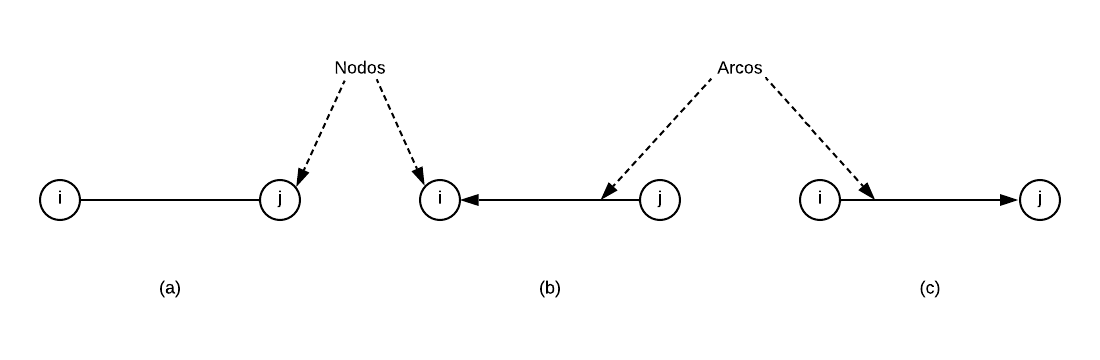
\includegraphics[width=17cm]{arcos_y_nodos.png}}
% \caption{(a) Arco no dirigido. (b) y (c) Arcos dirigidos.}
% \label{fig:arcos_y_nodos}
% \end{figure}

% Una secuencia de arcos que conectan dos nodos se denomina cadena. Cada arco en una cadena comparte exactamente un nodo con el arco anterior.

% Cuando todos los arcos de una cadena se dirigen de tal manera que es posible atravesar la cadena en las direcciones de los arcos desde el nodo de inicio hasta el nodo final, se denomina camino. En la ``Fig.~\ref{fig:caminos}'' se observan dos caminos de A a D:

% \begin{enumerate}
%     \item ABCD
%     \item ABEFD
% \end{enumerate}

% \begin{figure}[H]
% \centerline{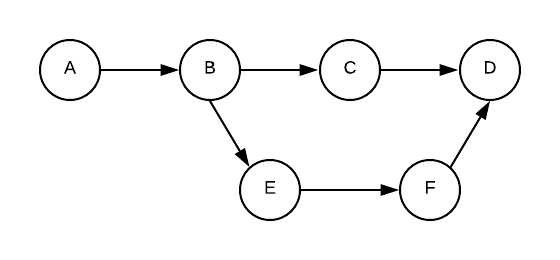
\includegraphics[width=8cm]{Caminos.png}}
% \caption{Caminos}
% \label{fig:caminos}
% \end{figure}

\section{Optimización}

% La optimización es una herramienta importante en la ciencia de la decisión y en el análisis de los sistemas físicos. Para usarlo, se debe identificar algún objetivo, una medida cuantitativa del rendimiento del sistema en estudio. Este objetivo podría ser el beneficio, el tiempo, la energía potencial o cualquier cantidad o combinación de cantidades que se puedan representar con un solo número. El objetivo depende de ciertas características del sistema, llamadas variables o incógnitas. Nuestro objetivo es encontrar valores de las variables que optimicen el objetivo. A menudo las variables están restringidas de alguna manera \citep{Nocedal1999NumericalOptimization}.
La optimización es una herramienta importante en la ciencia de la decisión y en el análisis de los sistemas físicos. Los problemas de optimización se componen generalmente de estos tres componentes \citep{Ramos2010ModelosOptimizacion}:

\begin{itemize}
    \item Función objetivo: Es la medida cuantitativa del funcionamiento del sistema que se desea optimizar (maximizar o minimizar).
    \item Variables: Representan las decisiones que se pueden tomar para afectar el valor de la función objetivo.
    \item Restricciones: Representan el conjunto de relaciones (expresadas mediante ecuaciones e inecuaciones) que ciertas variables están obligadas a satisfacer.
\end{itemize}

El modelado de un problema dado consiste en el proceso de identificar el objetivo, variables y restricciones. La construcción de un modelo es el primer paso para el proceso de optimización, luego se utiliza un algoritmo para encontrar su solución. Existen numerosos algoritmos, cada uno de los cuales se adapta a un tipo particular de problema de optimización \citep{Nocedal1999NumericalOptimization}.

Después de que se haya aplicado un algoritmo de optimización al modelo, debemos ser capaces de reconocer si ha tenido éxito en su tarea de encontrar una solución. En muchos casos, hay expresiones matemáticas que se conocen como condiciones de optimalidad para verificar que el conjunto actual de variables sea la solución del problema. Finalmente, el modelo puede mejorarse aplicando técnicas como el análisis de sensibilidad, que revela la sensibilidad de la solución a los cambios en el modelo y los datos \citep{Nocedal1999NumericalOptimization}.

Un modelo es infactible cuando no existen soluciones que satisfagan todas las restriciones. Esto puede ocurrir debido a que la formulación es incorrecta o los datos no son los correctos.

% \section{Formulación matemática}

% La optimización es la minimización o maximización de una función sujeta a restricciones en sus variables.

La formulación matemática para un problema de optimización puede ser descrito como sigue:

\begin{equation} \label{min}
\min_{x \in \mathbb{R}^n} f(x) 
\end{equation} 

sujeto a 

\begin{equation} \label{sujeto}
\begin{aligned}
    c_{i}(x) = 0, i \in \xi \\
    c_{i}(x) \geq 0, i \in \mathcal{I}
    \end{aligned}
\end{equation}

Aquí $f$ y cada $c_{i}$ son funciones de valores escalares de las variables $x$. $\mathcal{I}$ y $\xi$ son conjuntos de índices.

En (\ref{min}) y (\ref{sujeto}) se utiliza la siguiente notación:

\begin{itemize}
    \item $x$ es el vector de variables, es decir, variables o desconocidos.
    \item$f$ es la función objetivo, una función de $x$ que queremos minimizar o maximizar.
    \item$c$ es el vector de restricciones que las variables deben satisfacer. Esta es una función vectorial de las variables $x$. El número de componentes en $c$ es el número de restricciones individuales que colocamos en las variables.
\end{itemize}

Los métodos de optimización los podemos clasificar en: métodos clásicos y métodos metaheurísticos. Dentro de los primeros se encuentra la optimización lineal, lineal entera mixta, no lineal, estocástica, dinámica. En el segundo grupo se incluyen los algoritmos evolutivos (genéticos, entre otros), el método del recocido simulado (SA), las búsquedas heurísticas (método tabú, búsqueda aleatoria, avariciosa, etc.) o los sistemas multiagente. \citep{Ramos2010ModelosOptimizacion}.

Los problemas de optimización se pueden clasificar según diferentes enfoques. Uno de los enfoques está basado en los valores permitidos para las variables de decisión, donde los problemas de optimización pueden clasificarse como problemas de programación entera o problemas de programación de valores reales \citep{Rao2009EngineeringEdition}.

Si algunas o todas las variables de decisión $x_1$, $x_2$,...$x_n$, solo pueden tomar valores enteros (o discretos), el problema es uno de programación de enteros. Por otro lado, si todas las variables de decisión pueden tomar cualquier valor real, el problema de optimización se denomina problema de programación de valor real.

\subsection{Programación entera (IP)}

Los tipos de programas enteros pueden clasificarse en:
\begin{itemize}
    \item Programas lineal de enteros mixtos (MILP): $x_i \geq 0$ y entero para algunas o todas las $i$. 
    \item Programas enteros puros: $x_i \geq 0$ y entero para cada $i$.
    \item Programas enteros 0-1: $x_i \in \{0,1\}$ para cada $i$.
\end{itemize}

La Figura \ref{fig:milp} muestra el espacio de solución factible en el área $S$ de un MILP, donde la variable de decisión $x$ corresponde a un valor entero mientras que la variable de decisión $y$ representa una variable continua. Por otra parte, en la Figura \ref{fig:pil} se representan mediante puntos a los posibles valores solución en el área $S$, donde ambas variables $x_1$ y $x_2$ corresponden a valores enteros.

\begin{figure}[H]
   \captionsetup[figure]{labelformat=empty}
   \centering
       \subfigure[][]{
            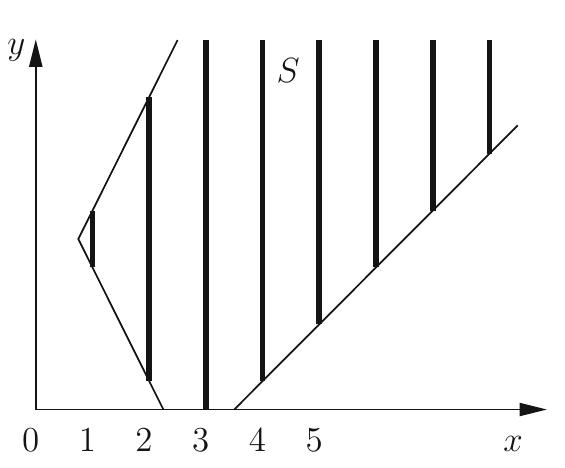
\includegraphics[width=0.45\textwidth]{milp.png}
            \label{fig:milp}
        }
        \subfigure[][]{
            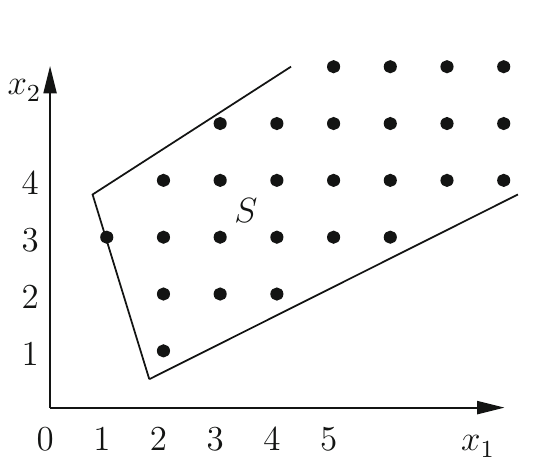
\includegraphics[width=0.45\textwidth]{pil.png}
            \label{fig:pil}
        }
   \caption{Espacion de solución factible. (a) Conjunto lineal de enteros mixto. (b) Conjunto lineal entero puro. [Fuente: \cite{Conforti2014IntegerProgramming}]}
   \label{fig:milp_ip}
\end{figure}

Una programación lineal entera pura es un problema de la forma:

\begin{equation} \label{programacion_entera}
\begin{aligned}
             \max\: & \mu x \\ 
        sujeto\:a\: & Ax \leq b \\
                    &\: x \geq 0\: entero
\end{aligned}
\end{equation}

donde los datos, generalmente racionales, son el vector fila $\mu = (\mu_1,...,\mu_n)$, la matriz $mxn$ $A=(a_{ij})$, y el vector columna $b=(b_1,..., b_m)$. El vector columna $x=(x_1,...,x_n)$ contiene las variables a ser optimizadas. Se dice que un $n$-vector $x$ es entero cuando $x \in \mathbb{Z}^n$. El conjunto $S := \{x \in \mathbb{Z}^n_+ : Ax \leq b\}$ de soluciones factibles de (\ref{programacion_entera}) es llamado el conjunto lineal entero puro \citep{Conforti2014IntegerProgramming}.

\subsection{Métodos para resolver la programación entera}

% 1.4. Métodos de Programación Integral
A pesar de que un IP limitado tiene solo un número finito de solución factible, la naturaleza entera de las variables dificulta la creación de un algoritmo efectivo que busque directamente entre los puntos enteros factibles del espacio de la solución. En vista de esta dificultad, los investigadores han desarrollado un procedimiento de solución que se basa en explotar el tremendo éxito en la resolución de problemas de LP. La estrategia para este procedimiento se puede resumir en tres pasos:

\begin{enumerate}
    \item Relaje las restricciones de enteros del IP para que el IP se convierta en un LP regular.
    \item Resuelva el modelo LP ``relajado'' resultante e identifique su punto óptimo (continuo).
    \item A partir del punto óptimo continuo, agregue restricciones especiales que forzarán iterativamente el punto extremo óptimo del modelo LP resultante hacia las restricciones enteras deseadas.
\end{enumerate}

Existen dos métodos ampliamente utilizados para generar restricciones especiales que forzarán el punto óptimo del problema de LP relajado hacia la solución entera deseada:

\begin{enumerate}
\item Plano de corte (\textit{Cutting plane}).
\item Ramificación y Acotación (\textit{Branch and bound}).
\end{enumerate}

En ambos métodos, la restricción agregada eliminará partes del espacio de solución relajada, pero nunca ninguno de los puntos enteros factibles. No se puede afirmar que ninguno de los dos métodos sea uniformemente más efectivo para resolver los IP. Sin embargo, los métodos de \textit{branch and bound} son mucho más exitosos computacionalmente que los métodos de plano de corte. Por este motivo, la mayoría de los códigos comerciales se basan en el uso del procedimiento de \textit{branch and bound}.

%definir modelo relajado

% \subsubsection{Algoritmos de Ramificación y Acotación (\textit{branch and bound})}

% Este método comienza relajando el requisito de enteros y tratando el problema como uno de programación lineal (LP, \textit{Linear Programming}). Si todas las variables toman valores enteros, la solución está completa. Si no, el algoritmo comienza una búsqueda de árbol.

% \subsubsection{Algoritmos de Planos de Corte}

% \subsubsection{Algoritmos de Ramificación y Corte (\textit{branch and cut})}

% Este método es un algoritmo exacto que consiste en una combinación de un método de plano de corte y un algoritmo de branch and bound.

% \subsubsection{Algoritmos Heurísticos}

